\subsection{Адаптер~--- аппроксимация векторного представления} 
\label{section:adapter_defenition}
Как отмечалось в секции $\ref{section:problem_statement}$, главная проблема при использовании оценочной модели $g_{\text{toxic}}$ в качестве функции потерь является отсутствие дифференцируемости по параметрам детоксификатора $\theta$.
Предлагается избавиться от явной генерации нейтрального предложения $s_{\text{detox}}$ детоксификатором для оценки степень токсичности получившегося предложения.

Введём произвольное предложение $s \in T \cup D$ и операцию $\textbf{one-hot}_{g}$ такую, что 
\begin{gather*}
    \textbf{one-hot}_{g}: V_{g} \to \{0, 1\}^{|V_{g}|}, \\ 
    \left(\textbf{one-hot}_{g} (i)\right)_{j = i} = 1, \\ 
    \left(\textbf{one-hot}_{g} (i)\right)_{j \not= i} = 0. 
\end{gather*}
Также введём матрицу входных эмбеддингов оценочной модели $E_g$. 
\textit{Эмбеддингом токена} называется его векторное представление, причём $E_g \in \mathbb{R}^{|V_g| \times e_g}$, где $e_g$~--- размер входных эмбеддингов оценочной модели.

Оценочная модель $g_{\text{toxic}}$ принимает на вход токены $\tau_{g}(s)$ сопоставляя им эмбеддинги из матрицы эмбеддингов $E_g $.
Эту операцию можно записать следующим образом:
\begin{gather*}
    O_{g} E_g \in \mathbb{R}^{n \times e_g}, \\
    O_{g} \in \{0, 1\}^{n \times |V_g|},
\end{gather*}
где $i$-я строчка в матрице $O_{g}$ есть one-hot вектор для $i$-го токена  $\tau_{g}(s)$.

Выход детоксификатора $f_{\theta}\bigl(\tau_{f}(s)\bigr) \in [0, 1]^{n \times |V_f|}$, как было описано в секции $\ref{section:machine_translation}$, есть распределение вероятностей токенов из $V_{f}$.
Введём \textit{адаптер} $A \in \mathbb{R}^{|V_f| \times e_{g}}$, апроксимирущий входные эмбеддинги оценочной модели следующим образом:
\begin{equation}\label{eqn:adapter_property}
    f_{\theta}\bigl(\tau_{f}(s)\bigr) A \approx O_{g} E_{g}.\tag{$\star$}
\end{equation}
При фиксированных параметрах оценочой модели это эквиваленто записи: 
\begin{gather*}
    g_{\text{toxic}}^{*} \bigl( f_{\theta}\bigl(\tau_{f}(s)\bigr)\bigr) 
    \approx g_{\text{toxic}} \bigl(\tau_{g} (s) \bigr), \\
    g_{\text{toxic}}^{*}: [0, 1]^{n \times |V_{f}|} \to [0, 1],
\end{gather*}
где $g_{\text{toxic}}^{*}$~--- оценочная модель $g_{\text{toxic}}$, в которой заменили входную матрицу эмбеддингов  $E_g$ на адаптер $A$.
Иллюстрация схемы работы изображена на рис. $\ref{fig:adapter_meaning_schema}$.
\begin{figure}[ht]
      \centering
      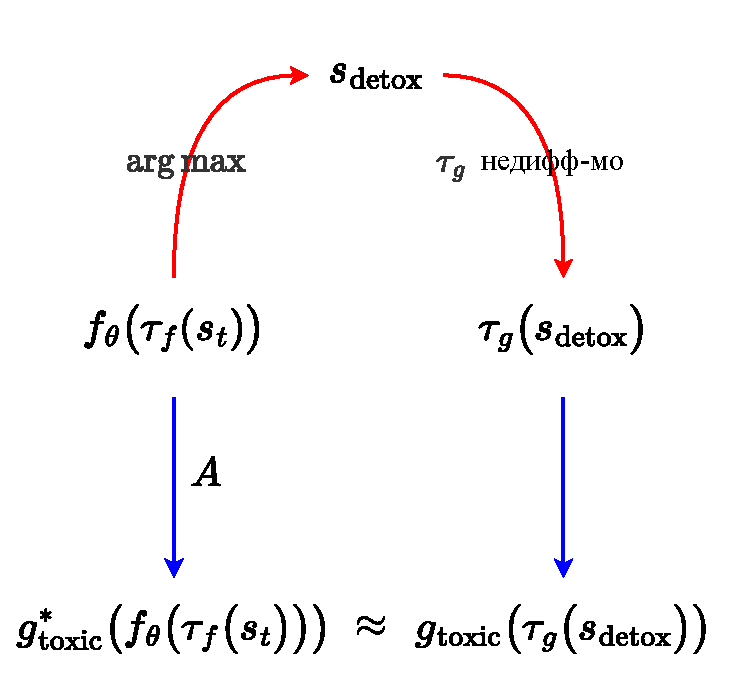
\includegraphics[width=0.66\textwidth]{images/non_diff_loss.pdf}
      \caption{
        Схема работы адаптера и решение проблемы дифференцируемости.
        Синими стрелками изображены операции не нарушающие  дифференцируемость, красными - нарушающие.
      }
      \label{fig:adapter_meaning_schema}
\end{figure}

В таком подходе можно интерпретировать выходное распределение детоксификатора $f_{\theta}\bigl(\tau_{f}(s)\bigr)$, как "зашумлённые" one-hot вектора.
Так как матрица эмбеддингов до этого принимала вектора со значениеями в $\{0, 1\}$, а теперь принимает со вектора значениемями на непрерывном отрезке $[0, 1]$.  
По сути в таком подходе строится взвешенная сумма эмбеддингов всех токенов словаря $V_{f}$. 

\subsection{Обучение адаптера} 
\label{section:adapter_training}
Пусть обучаемые параметры~--- это только параметры адаптера $A$, все остальные параметры $g_{\text{toxic}}^{*}$ фиксированы, как и параметры $g_{\text{toxic}}$.
Также будем считать, что имеется обученная модель кодировщик-декодировщик на задачу детоксификации $f_{\theta}$, как это было описано в секции $\ref{section:machine_translation}$. 

Пусть имеется пара предложений $s_t, s_d$~--- токсичное и его нейтральный вариант соответственно. 
Введём две вероятности токсичности: 
\begin{align*}
    P_{\text{toxic}} &= g_{\text{toxic}} \bigl(\tau_{g}(s_d) \bigr), \\
    P^{*}_{\text{toxic}} &= g^{*}_{\text{toxic}} \bigl(f_{\theta} \bigl(\tau_{g}(s_t)\bigr) \bigr). 
\end{align*} 
Как было описано в предыдущей секции, мы требуем от адаптера выполнения аппроксимации \eqref{eqn:adapter_property}. 
Но явно задавать функцию потерь для выполнения этого свойства не разумно, так как мы хотим использовать выход оценочной модели, а не только выход эмбеддинг слоя.
Поэтому требуется выполнения аппроксимации на выход моделей: $P_{\text{toxic}} \approx P^{*}_{\text{toxic}}$. 

Дабы достичь требуемого свойства аппроксимации определим функцию потерь для обучения адаптера, как дивергенцию Кульбака-Лейблера:
\begin{gather*}
    D_\text{KL} \left(P_{\text{toxic}} \parallel P^{*}_{\text{toxic}} \right) 
    = P_{\text{toxic}} \cdot \log\left(\frac{P_{\text{toxic}}}{P^{*}_{\text{toxic}}}\right) 
    + \left(1 - P_{\text{toxic}} \right) \cdot \log\left(\frac{1 - P_{\text{toxic}}}{1 - P^{*}_{\text{toxic}}}\right).
\end{gather*}
Тогда при обучении адаптера требуется решить следующую задачу:
\begin{gather*}
    D_\text{KL}\left(P_{\text{toxic}} \parallel P^{*}_{\text{toxic}} \right) \longrightarrow \min_{A}.
\end{gather*}
Причём важно отметить, что все параметры оценочной модели и модели-детоксификатора являются фиксированными.
Схема обучения адаптера изображена на рис. $\ref{fig:adapter_training_schema}$.
\begin{figure}[ht]
      \centering
      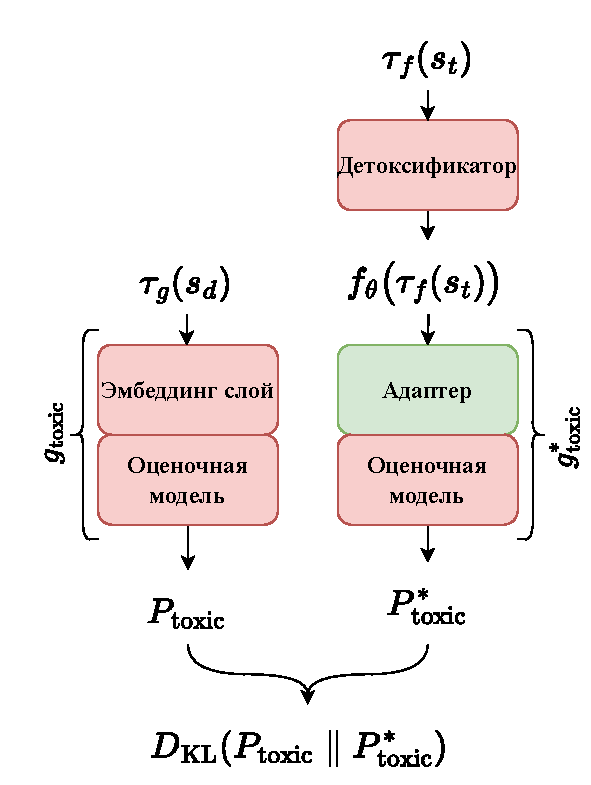
\includegraphics[width=0.66\textwidth]{images/adapter_train.pdf}
      \caption{
        Схема обучения адаптера.
        Красными блоками изображены фиксированные параметры моделей.
        Зелёным~--- обучаемые параметры. 
        В данном случае только параметры адаптера.
    }
      \label{fig:adapter_training_schema}
\end{figure}

\subsection{Использование адаптера в дообучении детоксификатора}
\label{section:posttrain}
В этой секции будем считать, что имеется обученный детоксификатор $f_{\theta}$ на задачу машинного перевода и адаптер $A$ для модели $g^{*}_{\text{toxic}}$.
Отметим, что адаптер был обучен для фиксированных параметров детоксифакатора. 
Поэтому при дообучении детоксификатора будет инвалидироваться результат обучения адаптера, так как адаптер обучался для других параметров детоксификатора.
Дабы избежать этого, требуется модифицировать алгоритм дообучения детоксификатора. 
Основная идея предложенной модификации основана на обучении порождающих моделей \cite{10.5555/2969033.2969125}.

Введём следующие обозначения:
\begin{align*}
    \text{CE} &= \mathcal{L}_{\text{CE}},\\
    \text{TP} &= P^{*}_{\text{toxic}}.
\end{align*}
Введём \textit{агрегирующую функцию потерь} $\mathcal{F}: \mathbb{R}^2 \to \mathbb{R}$, которая будет принимать значения кросс-энтропии $\mathcal{L}_{\text{CE}}$ и вероятности токсичности $P^{*}_{\text{toxic}}$.
Тогда предложенный алгоритм можно описать следующим образом: 
\begin{enumerate}
    \item $N$ батчей обучается детоксиификатор $f_{\theta}$, минимизируя функцию потерь $\mathcal{F} (\text{CE}, \text{TP})$, при фиксированных параметрах адаптера $A$.
    \item $M$ батчей обучается адаптер $A$, минимизируя $D_{\text{KL}}$, как описано в секции $\ref{section:adapter_training}$, при фиксированных параметрах детоксификатора $f_{\theta}$. 
\end{enumerate}